\documentclass[a4paper,11pt, oneside]{report}

% Package import
\usepackage[a4paper,inner=3.5cm,outer=2.5cm]{geometry}
\usepackage[english,american]{babel}

\usepackage{latexsym}
\usepackage[T1]{fontenc}
\usepackage[utf8]{inputenc}
\usepackage{graphicx}
\usepackage{hyperref}
\usepackage{tabularx}
\usepackage{etoolbox}
\usepackage{fancyhdr}
\usepackage{amsthm}
\usepackage{mathtools}
\usepackage[xindy]{glossaries}
\usepackage{hyperref}
\usepackage{lastpage}

% clear default
\fancyhead{}
\fancyfoot{}

\pagestyle{fancy}
\fancyhf{}
\renewcommand{\headrulewidth}{0pt} % optional
\fancyfoot[L]{Chapter: \nouppercase{\leftmark}}
\fancyfoot[R]{\thepage/\pageref{LastPage}}

% Redefine the plain page style, Chpater page
\fancypagestyle{plain}{%
  \fancyhf{}
  \renewcommand{\headrulewidth}{0pt} % optional
  \fancyfoot[R]{\thepage/\pageref{LastPage}}
}

\renewcommand{\chaptermark}[1]{\markboth{\MakeUppercase{#1}}{}}

% Glossar
\newglossaryentry{ATAS}
{
    name=ATAS,
    description={Aplinist Tracker \& Alerting System}
}

\theoremstyle{definition}
\newtheorem{exmp}{Beispiel}[subsection]


\makeglossaries

\setcounter{secnumdepth}{2}
\setcounter{tocdepth}{1}

\begin{document}
\pagestyle{empty} %Keine Kopf-/Fusszeilen auf den ersten Seiten.
\begin{titlepage}
\begin{center}

% Oberer Teil der Titelseite:
\includegraphics[width=0.08\textwidth]{img/bfh_logo.png}\\[1cm]    
\textsc{\LARGE Bern University of Applied Sciences}\\[1.5cm]
\textsc{\Large Project 2}\\[0.5cm]

% Title
\newcommand{\HRule}{\rule{\linewidth}{0.3mm}}
\HRule \\[0.4cm]
{\huge Aplinist Tracker \& Alerting System}\\[0.3cm]
{\huge \bfseries  ATAS}
\HRule \\[2cm]

\includegraphics[width=0.2\textwidth]{img/atas_logo.png}\\[3cm]    

% Author und Lehrer
\begin{minipage}{0.4\textwidth}
\begin{flushleft} \large
\emph{Author:}\\
Martin \textsc{Schmidli}\\
\end{flushleft}
\end{minipage}
\hfill
\begin{minipage}{0.4\textwidth}
\begin{flushright} \large
\emph{Teacher:} \\
Mohamed \textsc{Mokdad}
\end{flushright}
\end{minipage}
\vfill

% Unterer Teil der Seite
Bern, {\large \today}
\end{center}
\end{titlepage}
\pagestyle{fancy}

\tableofcontents

\chapter{Project description}

\section{Introduction}
The Alpinist Tracker and Alerting system short ATAS has two main functionalities.
\begin{enumerate}
\item Track peobles location which are located on a mountain for example skiers, hikers... short called alpinists.
\item Alarm a rescue team if the alpinist had an accident
\end{enumerate}


\newpage
\section{Systemarchitecture, Abstract}
This section will provide an abstract overview which kind of components are used in the ATAS System.\\
The sytem will be devided into different modules. All the modules and users of the system are explained on the next page.\\

\includegraphics[width=0.93\textwidth]{img/ATAS_SystemOverview_Abstract.png}

\subsection{System Users}
\subsubsection{Alpinist}
Generalization: Skier, hiker or any other person in the mountains.
\subsubsection{Administrators}
The administrators of the system are peoble working for a tourism region, hospital or rescue teams like the Rega.

\subsection{System Modules}
\subsubsection{Tracker}
Imagine a small mobile device, following called \textbf{tracker}. The Tracker can be carried by an \textbf{alpinists} for example in a bagpack.\\[0.3cm]
The tracker device is equipped with an \textbf{alarm-button} and a \textbf{speaker}. With the alarm-button, the alpinist can inform the administrators about an accident. For example if the alpinist broke its knee.\\[0.3cm]
The speaker is used to inform the alpinist, with an alarming sound, that he's situated inside a dangerzone and he would better leave this zone immediately. A dangerzone is a place with a high possibility for an accident, for example, an area with a high possibility for an avalanche.\\[0.3cm]
The tracker is sending its GPS position to a receiver station, following called \textbf{gateway}. 
\subsubsection{Gateway}
A device which is able to talk to multible trackers. The gateway can be installed in a village/ building in the valley next to the mountains.\\[0.3cm]
All the gateway are sending the received locations from the trackers to a central datamanager called \textbf{broker}. 
\subsubsection{Broker}
The broker collects data and stores them. The Broker provides an Interface where the webapplication can grab all the data to present them.

\subsubsection{Webapplication}
The administrators can use a  \textbf{webapplication} / webpage to 
\begin{itemize}
\item
monitor the actual position of the persons on the mountains. 
\item
define dangerzones
\end{itemize}

\subsubsection{Logic}
Software / service which calculates if a tracker is inside a dangerzone. If the tracker is inside a dangerzone it will send an alarm to the tracker. The alarmsignal is relayed over the Broker.

\section{Usecase}
So why is the ATAS system useful?
The ATAS system can be used for:
\begin{itemize}
\item If an avalanche is triggered in the mountains, its position can be compared to the position of the trackers.
If at the time of the incident, a tracker was in this area, the rescue teams can be sent to do a rescue operation. This immediate action will give the victims important seconds and may save lifes.
\item If peoble were in the avalanche and the tracker survived, the device could keep sending data and support the rescue team in their mission bye pointing them to the location of the persons. If no transmission is possible through snow, the rescue team has at least its last GPS location, this might reduce the amount of time to find the person. ATAS is not planned as a replacement for avalanche transceivers, it should be seen as a supplement.
\item
If a tracker is moving towards a dangerzone, for example an area with rockfall, the user can be informed with the tracking device.
\item If an alpinist had an accident in the mountains, the person can send a rescue signal with the tracker device by triggering the alarm-button.
\end{itemize}

% TODO Use Case Diagram

\newpage

\section{Technologies}
At first glance this hole system must look very laborious  to a user. Why should a person have to take another device with him on his hikes? He could easily use his smartphone and an App to send his location. This statement is true if we consider only the touristic ski areas of switzerland. In most  ski areas the phone reception is wonderful. If we leave those ''safe'' areas and go to a higher altitude, the reception gets worse or disappears completely. \\[0.3cm]
This is the reason why for this project other technologies had to be found.\\[0.3cm]
For this project the following technologies were used:\\
MQTT, LoRA, LoRaWAN\\[0.3cm]
You should get yourself familiar with these technolgies to fully understand the following chapters.

\section{Demarcation}
This section defines which kind of tasks are to do during this project. These goals have been set by the project leader.
\begin{itemize}
\item Build a tracking device
	\begin{itemize}
		\item
			The alpinist should be able to trigger a manual alarm and inform the rescue team of an accident
		\item
			the tracker should track the position of the user and send the data to a data collector (broker)
	\end{itemize}
\item Build a webpage, which enables the administrators to
	\begin{itemize}
		\item
			view the location of the trackers
		\item
			manage dangerzones
	\end{itemize}
\item Build a software / service which controls the position of the trackers. If a tracker dwells inside a dangerzone the tracker has to be alerted.
\item Connect all the modules
\item Setup a broker system
\end{itemize}

% Chapter Systemarchitecture Detail
\chapter{Systemarchitecture}
This chapter will provide a detailed overview how the ATAS System was implemented. It will be more technical and show in detail how the modules of ATAS interact with each other.


\newpage
\noindent
\section{System Overview}
\includegraphics[width=0.9\textwidth]{img/ATAS_SystemOverview_Detail.png}

\newpage
\section{Tracker}
The tracker itself contains different components.

\subsection{Computer}
As my knowledge for hardware close porgramming (c, c++ ...) is failry limited, I decided to use a hardware plattform, which handles most of the system tasks for me. The computer had to be small and doesn't use to much energy. I decided to use a Raspberry Pie 3  single board computer.

\subsubsection{System Overview}
The Raspberry Pie is connected to other devices\\[0.3cm]
\includegraphics[width=\textwidth]{img/ATAS_SystemOverview_Tracker_Computer.jpg}

\subsubsection{Tasks}
The Raspberry Pie computer is used to
\begin{itemize}
\item Recieve GPS data from the GPS module via UART
\item Recieve and send data to the Lora Module via SPI
\item Listen for signals from the alert-button
\item Enables or disables the speaker
\end{itemize}

\subsubsection{Finished product}
The following pictures show the final tracker I built during this project\\[0.3cm]
Picture of the assembled tracker\\[0.3cm]
\includegraphics[width=\textwidth]{img/atas-tracker-assembled.jpg}
The alarm-button was placed on top of the case. All the other components are safely stored inside a case.
\newpage
\noindent
Picture of the disassembled tracker\\[0.3cm]
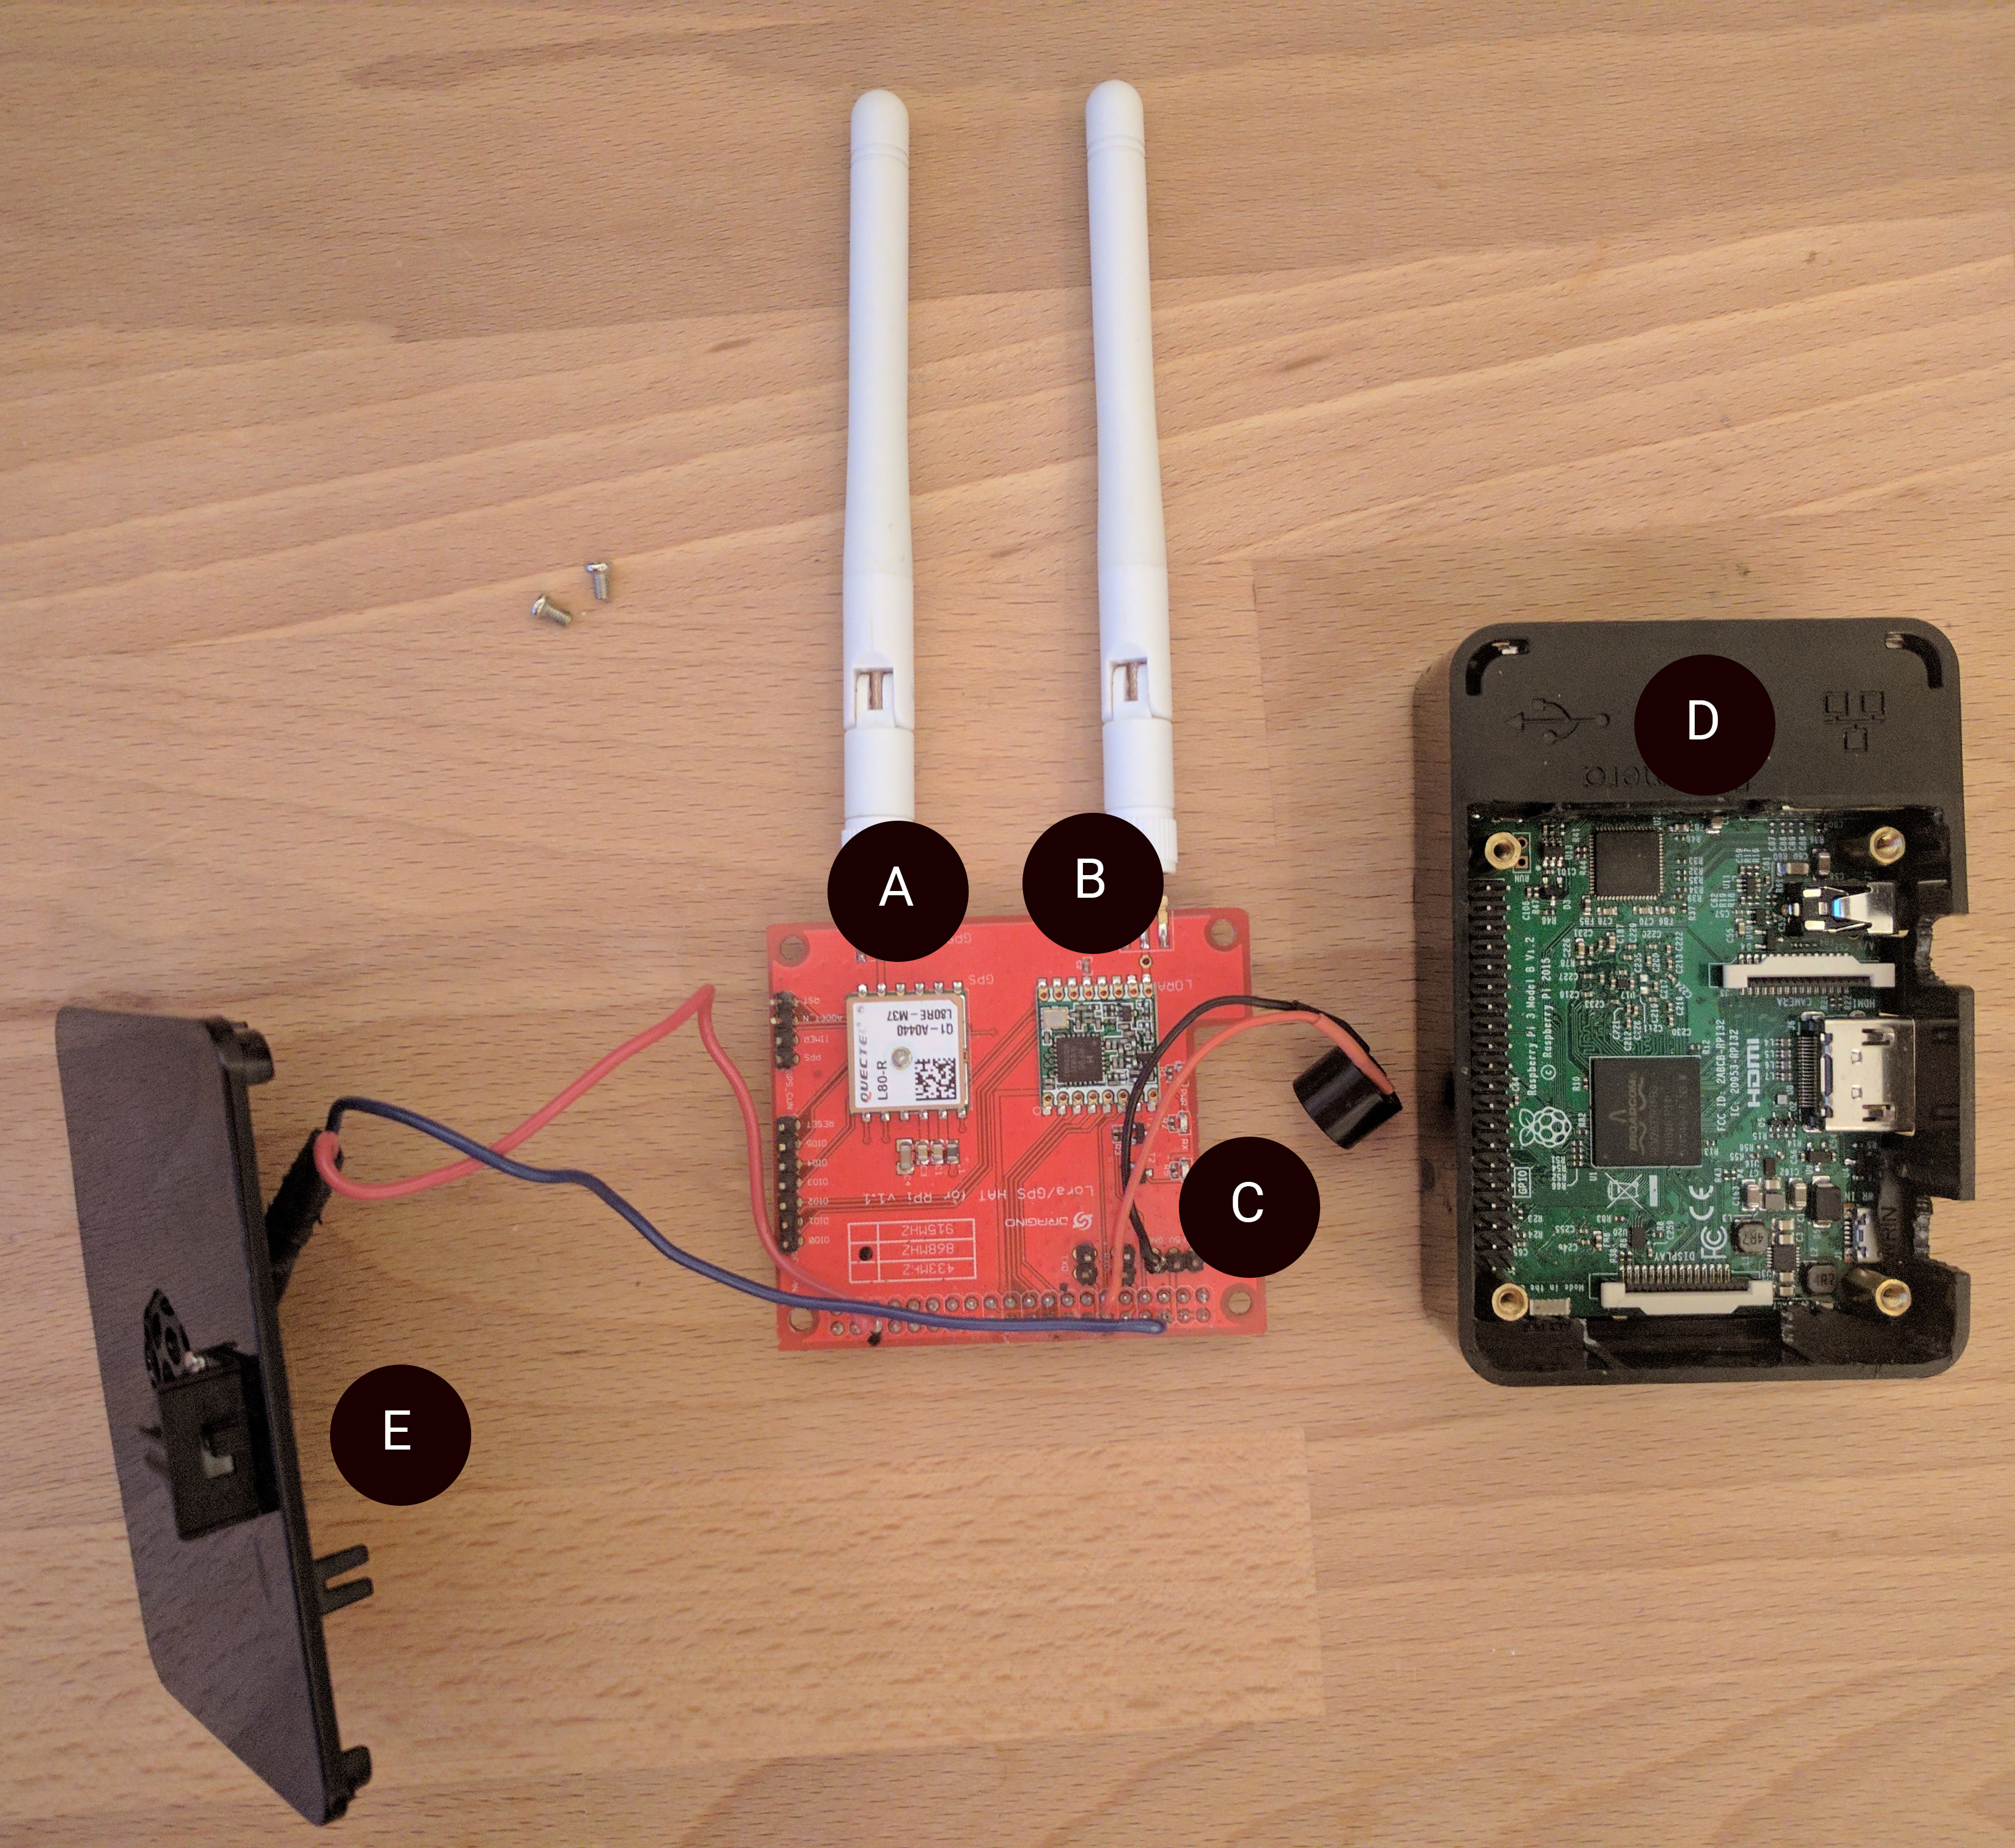
\includegraphics[width=\textwidth]{img/atas-tracker-disassembled.jpg}
\begin{itemize}
\item A: GPS Module with the corrsponding antenna
\item B: LoRa Module with the corresponding antenna
\item C: Piezo Speaker
\item D: Raspberry Pie computer
\item E: Alarm-button
\end{itemize}

\newpage
\subsection{Battery}
The tracker needs to mobile so we can put it in our backpack. To power the tracker I attached a battery pack over USB.\\[0.3cm]
Type: Aukey PB-Y3 Battery Pack\\
Power: 30000mAh\\
Physical Interface: Attached to the Raspberry Pie over Micro USB.
\subsubsection{Diagramm}
\includegraphics[width=0.95\textwidth]{img/ATAS_SystemOverview_Tracker_Battery.png}

\subsection{GPS Module}
The GPS Module provides the GPS location to the tracker.\\[0.3cm]
Type: MT3339\\
Interface:  Acessable via UART.
\subsubsection{Diagramm}
\includegraphics[width=0.95\textwidth]{img/ATAS_SystemOverview_Tracker_GPS.png}
\subsubsection{Tasks}
The GPS module will be used to
\begin{itemize}
\item Get the GPS Location(Longitude, Latitude) of the Tracker
\item Sends GPS data to the Raspberry Pie via UART
\end{itemize}


\subsection{LoraWan Modul}
The LoRaWan Modul establishes the wireless connection to a LoRaWan gateway.\\[0.3cm]
Type: LoRa Module Semtech SX1276\\
Interface: Acessable via SPI
\subsubsection{Diagramm}
\includegraphics[width=0.95\textwidth]{img/ATAS_SystemOverview_Detail_LoRaWan.png}

\subsubsection{Tasks}
The Lora module is used to
\begin{itemize}
\item Receive and transmit data to LoRaWan gateway.
\item Receive and transmit data to the Raspberry Pie over SPI.
\end{itemize}

\newpage
\subsection{Alarm Button}
A simple hardware switch. Can be put to On or Off.
\begin{itemize}
\item If the switch has been triggered by the aplinist, the GPIO input on the Raspberry Pie is set to Low (On / Alert) or High (Off / no Alert)
\item This simple switch gives the alpinist the possibility to trigger an alarm manually
\end{itemize}

\subsubsection{Diagramm}
\includegraphics[width=0.95\textwidth]{img/ATAS_SystemOverview_Detail_AlarmButton.png}

\subsection{Speaker}
A simple Piezo buzzer.
\subsubsection{Tasks}
\begin{itemize}
\item Gets enabled by the Raspberry Pie
\item Generates an alamring signal, which indicates, that the tracker is inside a dangerzone.
\end{itemize}

\subsubsection{Diagramm}
\includegraphics[width=0.95\textwidth]{img/ATAS_SystemOverview_Detail_Sound.png}

\newpage
\section{Gateway}
The gateway relays data between the trackers and The Things Network (TTN). What kind of fucntionality TTN is providing is explained later in this docuent.

\subsubsection{Diagramm}
\includegraphics[width=0.95\textwidth]{img/ATAS_SystemOverview_Detail_Gateway.png}

\subsubsection{Tasks}
The Lora Gateway will be used to
\begin{itemize}
\item Receive and transmit data to the Cloud Network The Things Network (TTN) over LoRaWan via TCP/IP
\item Sends and receive datat to the Trackers over LoRaWan via Lora
\end{itemize}

\newpage

\section{Broker}
The broker has been split up in subcomponents. The broker service hasn't been developed by myself. I use two platforms the Things Network (TTN) and CloudMQTT.

\subsection{The Things Network short TTN}
The Things Network short TTN is an internet platform whichs allows us to connect LoRaWan devices. TTN will send (Downlink) and receive (Uplink) data from the trackers via gateway. TTN will collect and store all the data which the gateways send to it. TTN provies a MQTT Broker to access the data more easily.

\subsubsection{Diagramm}
\includegraphics[width=\textwidth]{img/ATAS_SystemOverview_Detail_TTN.png}

\subsubsection{Tasks}
\begin{itemize}
\item Manage trackers
\item Manage gateways
\item Provides MQTT broker
\item Send and Receive data from the trackers via gateway
\end{itemize}

\newpage
\subsection{CloudMQTT}
To this date, the TTN MQTT broker does not provide the possibility to access the data via websocket interface. To bring MQTT over websocket to a  webapplication, another service was needed. I decided to setup CloudMQTT. \\[0.3cm]
CloudMQTT mirrors the TTN MQTT Broker Topics and provides an websocket interface. Our webapplication and the atas-service can use this interface to request and publish data from the trackers.\\[0.3cm]
All the data published to CloudMQTT are published to the TTN MQTT broker aswell. All the topics of the TTN broker are subscribed from the CloudMQTT service. 

\subsubsection{Diagramm}
\includegraphics[width=0.94\textwidth]{img/ATAS_SystemOverview_Detail_CloudMQTT.png}


\newpage
\section{Software}
\subsection{Atas-Service}
Atas-Service calculates if a tracker is inside a dangerzone. The service is comparing the GPS location of the tracker with the geographical area of the dangerzone. If the tracker is inside a dangerzone it will send an alarm to the tracker. The alarmsignal is send to the TTN Network over MQTT via CloudMQTT.\\[0.3cm]
Atas-Service provides a REST interface. Dangerzones created with the webapplication are sent to the atas-service over REST. This allows the webapplication to get and store the information about dangerzones. The database used in this project is a Mongo db.\\[0.3cm]
Atas-service is a node.js application written in Javascript.
\subsubsection{Diagramm}
\includegraphics[width=\textwidth]{img/ATAS_SystemOverview_Detail_atasservice.png}


\subsubsection{Process - MQTT Message arrives}
The flow chart  on the next page displays the process when a new MQTT message with GPS location data arrives. The flowchart doesn't represent the actual code. Dummy syntax /code was used to make the chart as understandable as possible.
\newpage
\includegraphics[width=0.88\textwidth]{img/atas-service-process-diagramm.png}\\

\newpage
\subsection{Atas-Web}
Atas-Web is the management interface of the ATAS System. Atas-Web is a webapplication. The application is written in Javascript and leverages the React.js library.\\[0.3cm]

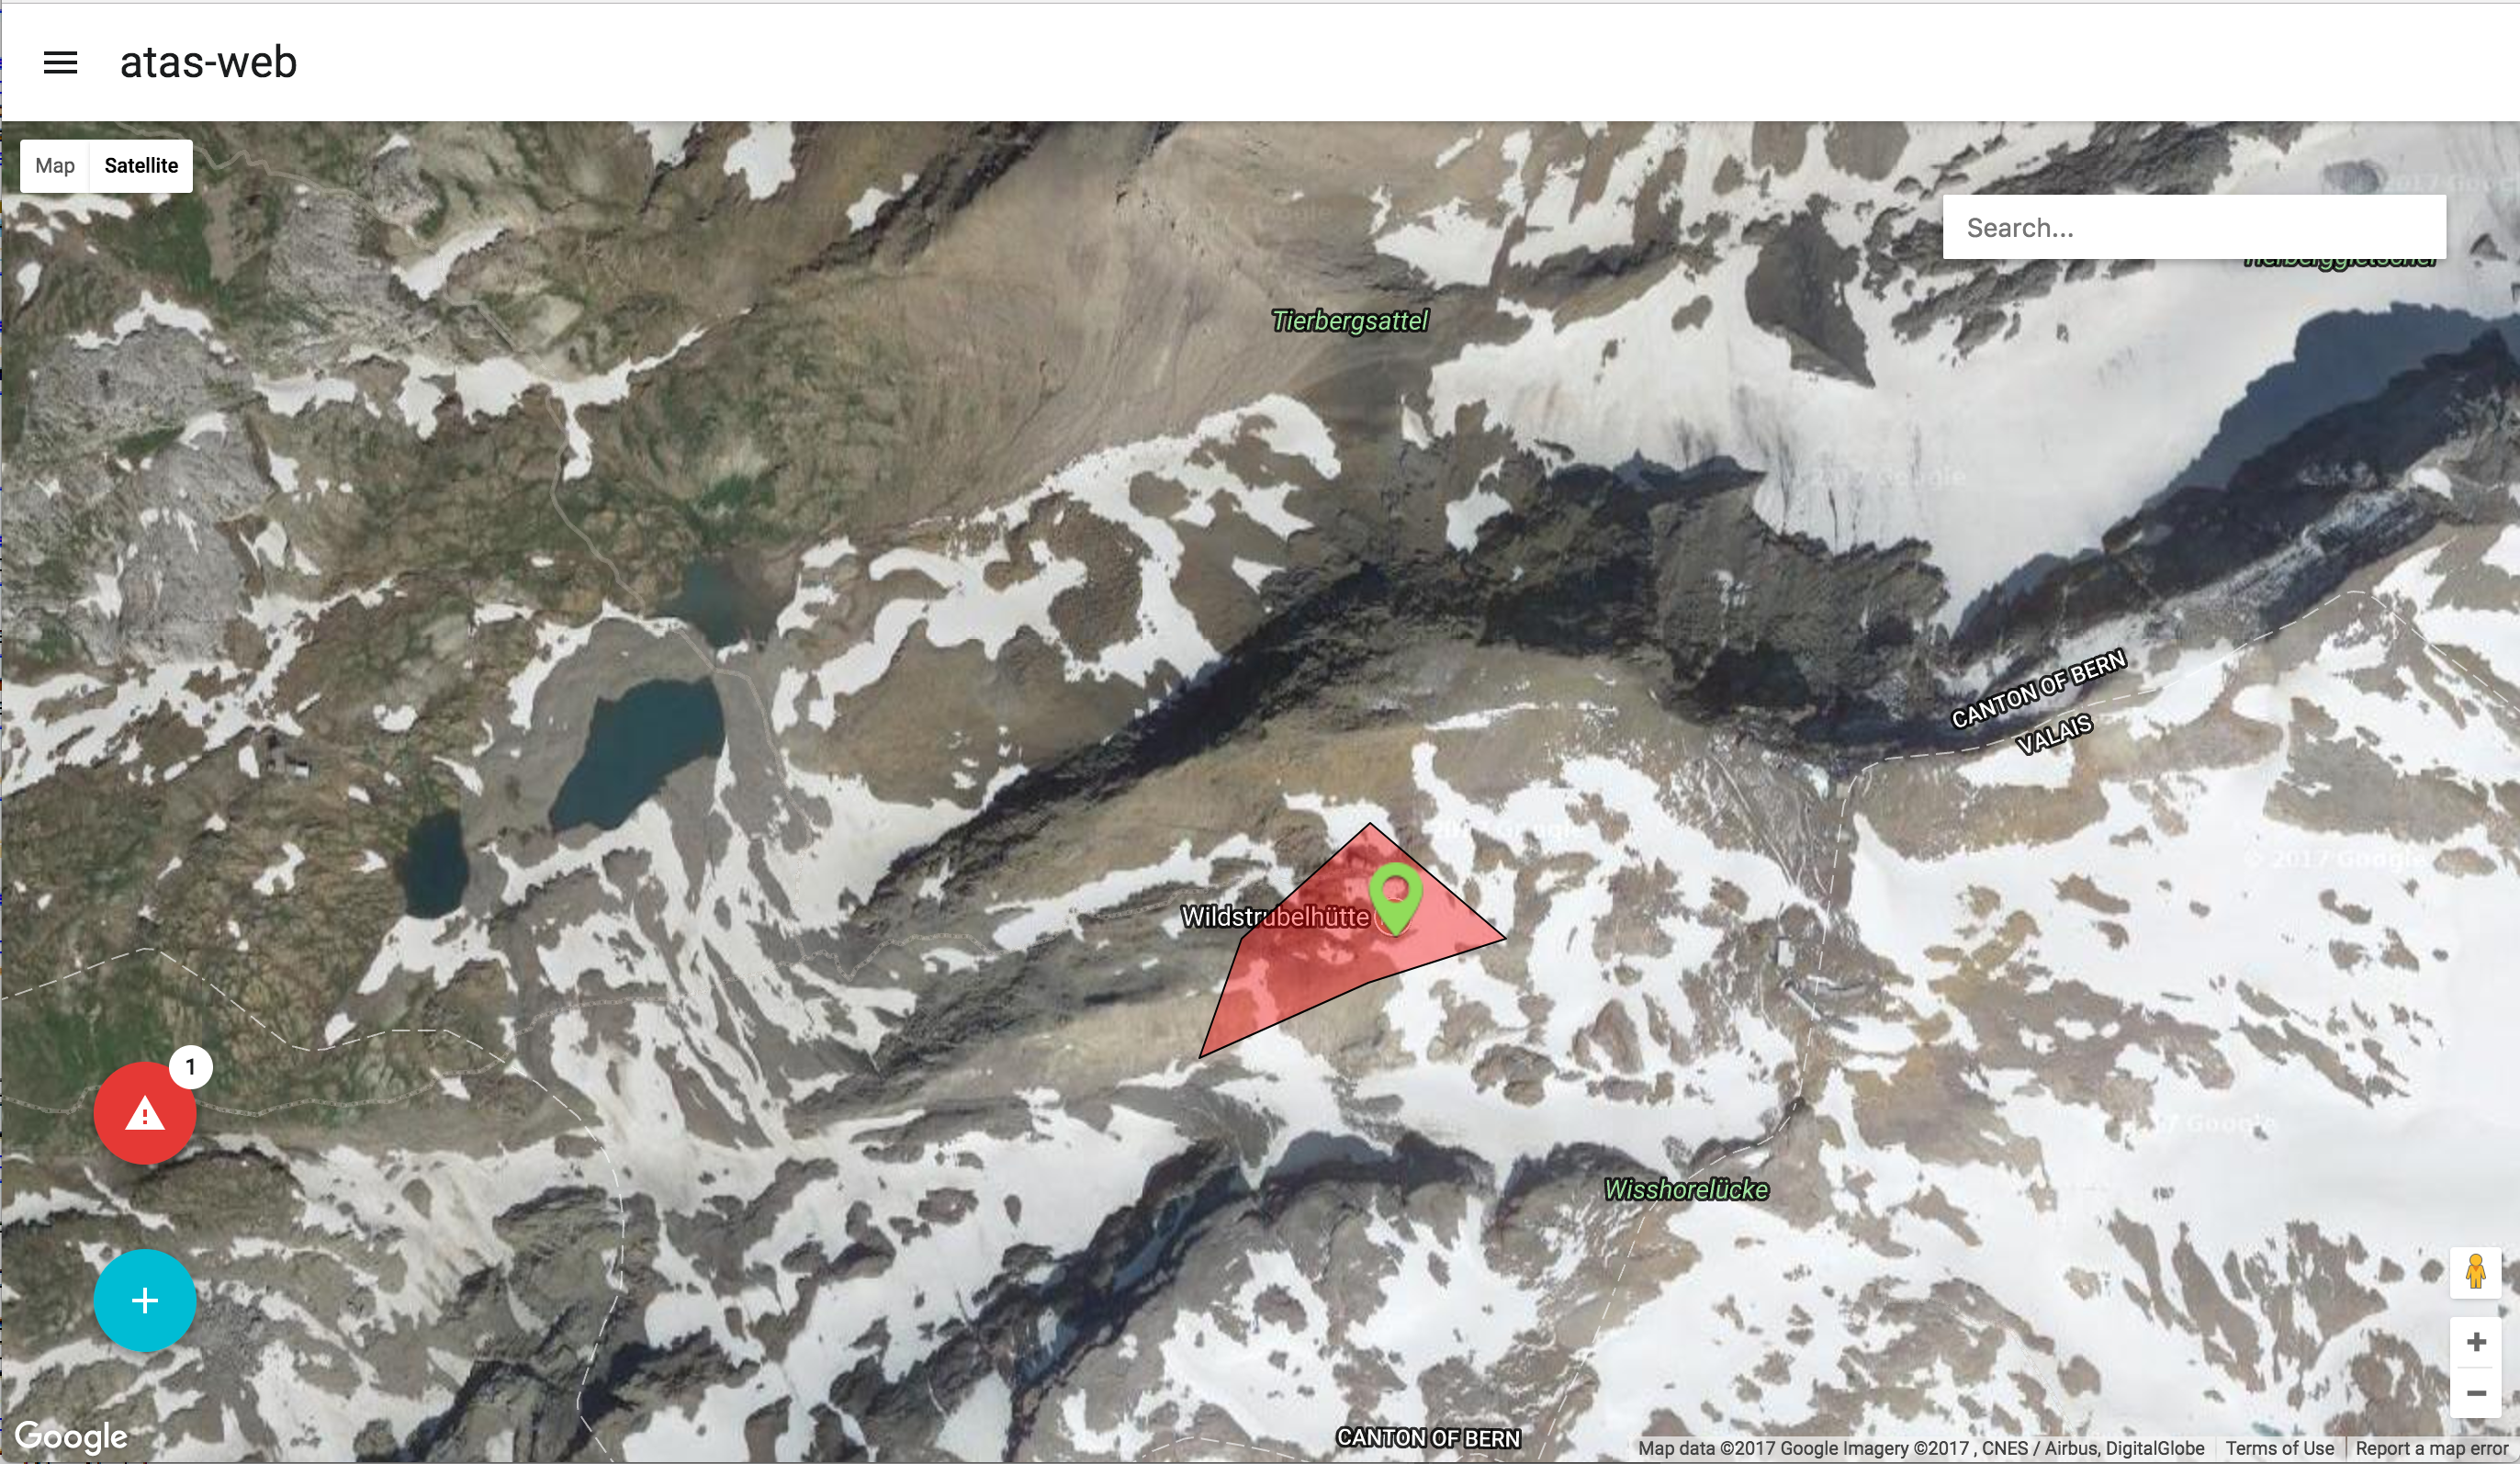
\includegraphics[width=\textwidth]{img/atas-web.png}

\newpage
\subsubsection{Functionality}

\begin{itemize}
\item \textbf{Map}\\ 
All the trackers are displayed on a world map. The trackers are displayed as a green symbol. If we click on a tracker, we see the actual GPS location.\\[0.3cm]
\includegraphics[width=\textwidth]{img/atas-web-map.png}

\item \textbf{Dangerzone Mangement} \\
We can easily create and delete dangerzones on the map. We can click on the Plus sign in the bottom left corner to change into the drawing mode\\[0.3cm]
\includegraphics[width=0.2\textwidth]{img/atas-web-adddangerzone.png}

\newpage
Once we switched in the drawing mode, we can draw a polygon which represents the dangerzone on the map.\\[0.3cm]

\includegraphics[width=0.5\textwidth]{img/atas-web-drawing.png}\\

An example of a drawn dangerzone. As we can see a tracker is inside the dangerzone.\\[0.3cm]
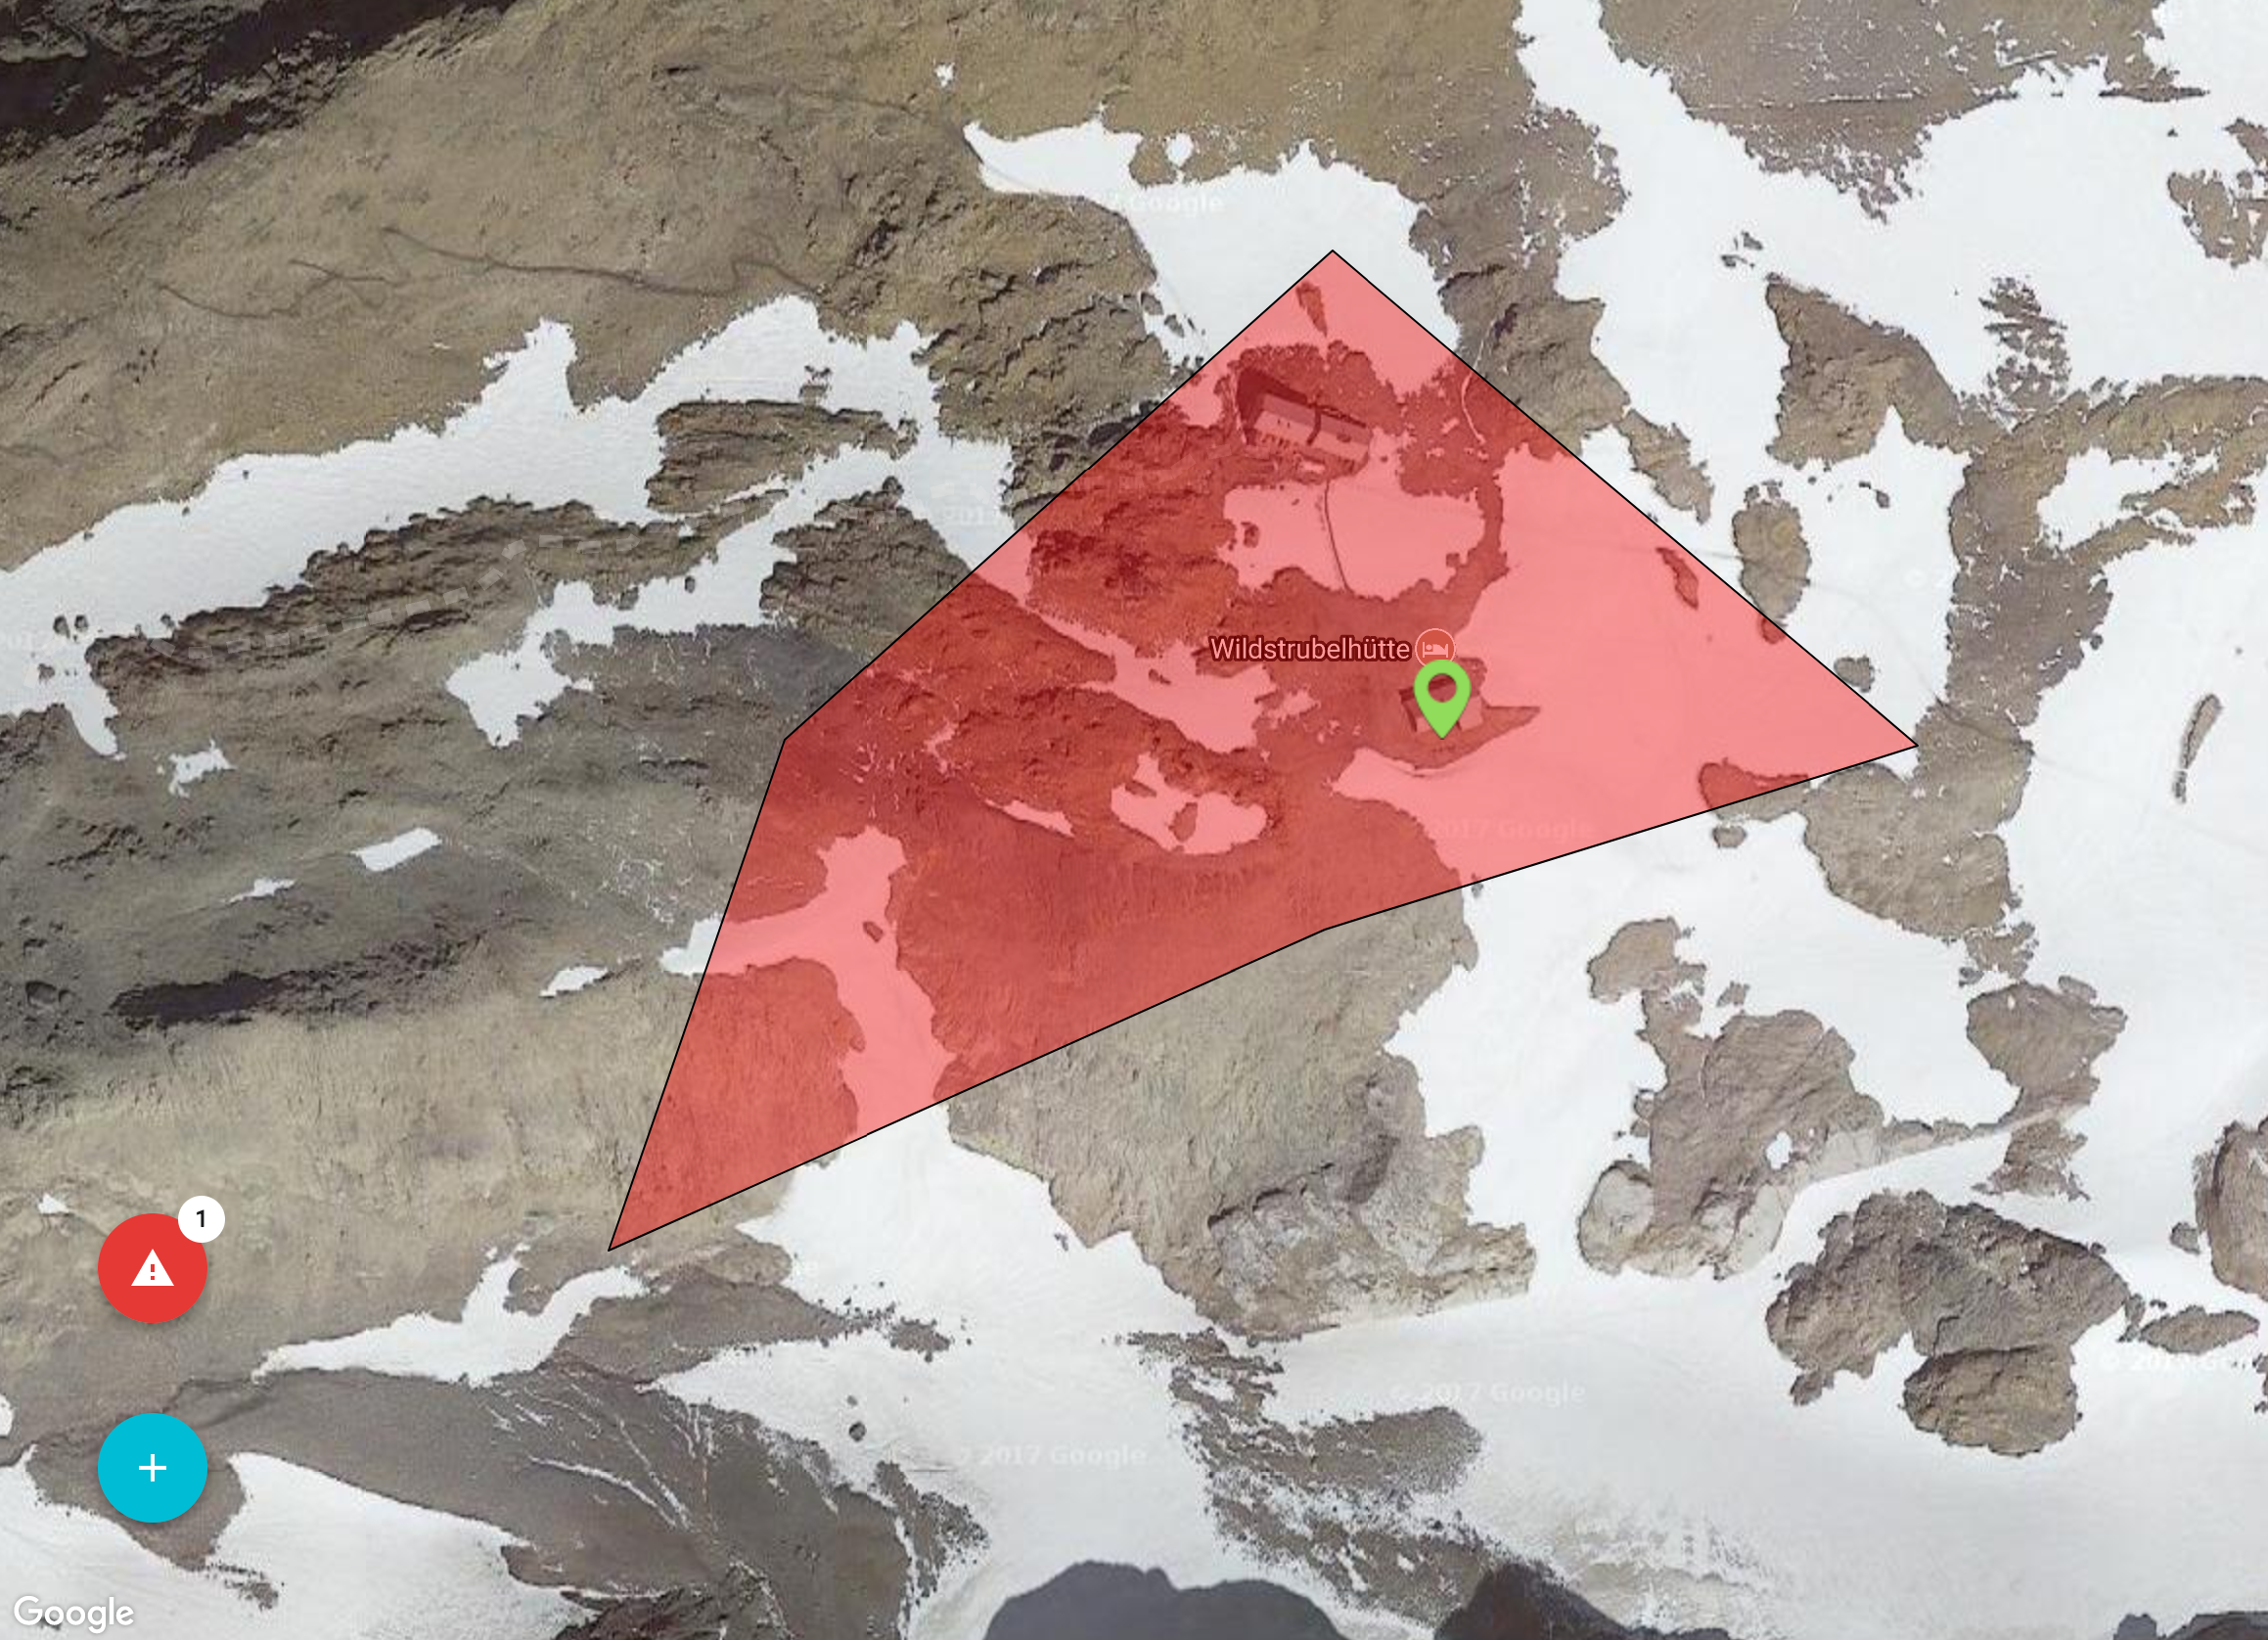
\includegraphics[width=0.9\textwidth]{img/atas-web-dangerzone.png}

\item \textbf{Alert View}\\ If we click on the Alert button\\[0.3cm]
\includegraphics[width=0.2\textwidth]{img/atas-web-alertbutton.png}\\[0.3cm]
we get an overview of all the alpinists requesting a rescue team and the trackers which resides inside a dangerzone.\\[0.3cm]
In this example the tracker atas-node45 resides inside a dangerzone.\\[0.3cm]
\includegraphics[width=\textwidth]{img/atas-web-alertoverview.png}\\

\newpage
\item \textbf{Search}\\
We can use the search bar to search for a location. Found locations are displayed as a yellow symbol.\\[0.3cm]
\includegraphics[width=\textwidth]{img/atas-web-search.png}\\

\end{itemize}

\newpage
  
\subsection{Atas-Node}  
Atas-Node is the software component running on the tracker computer. The software is written in c++.\\[0.3cm]
To make the communication between atas-node and the GPS Module as easy as possible I decided to install GPSD. GPSD is a daemon running on the linux Operating System on the tracker. GPSD provides us a simple interface and a c++ library to query the actual GPS position.

\subsubsection{Functionality}
For every task I created a separate class in c++.
\begin{itemize}
\item \textbf{Ataslora}\\
Handles the communication with the LoRaWan Module. Used for sending and receiving data
\item \textbf{Atasgps}\\
Handles the communication with the GPSD Deamon. Queries the GPS location.
\item \textbf{Atasbutton}\\
Initialized the GPIO PIN to act as an Input. Reads the GPIO levels, High or Low.
\item \textbf{Atassound}\\
Controls the Piezo speaker. Enables or disables the alarmsound.
\end{itemize}

\subsubsection{Process - Hole program}
On the next page you are going to see a flow chart of the atas-node programm. The flowchart doesn't represent the actual code. Dummy syntax /code was used to make the chart as understandable as possible.
\newpage
\includegraphics[width=0.88\textwidth]{img/atas-node-process}\\

\chapter{Dataflow}
\section{MQTT}
The following topic structure is used for the MQTT communication
\subsection{Topics}
\includegraphics[width=\textwidth]{img/ATAS_MQTT_Topic.png}

\newpage
\section{Tracker}
This section will describe which data is send and received by the tracker\\
\subsection{Tracker $\rightarrow$ TTN}
The tracker sends messages to the TTN via LoRaWan gateway.\\
A message contains 4 values.
\begin{itemize}
\item Latitude: GPS latitude of the tracker
\item Longitude: GPS longitude of the tracker
\item Button pressed: If the switch has been set to on the value is 1 otherwise the value is 0.
\item In Dangerzone: When a tracker is inside a dangerzone it will be informed by the atas-service (downlink). The tracker stores this informaton but also sends back the information to the TTN (uplink). This mechanism was developed to have an acknowledement from the trackerto check  if he received the alarm signal. The Value is 1 if the tracker is in a dangerzone and 0 if the tracker is not inside a dangerzone.
\end{itemize}
\includegraphics[width=\textwidth]{img/atas-tracker2ttn.png}\\

\chapter{Conclusion}
I had my concerns at the beginnen of this project as it required some know-how in electronic components, currenct flow and so on. As I'm an IT system engineer and not an electronics technician I always tried to avoid this topic, but im glad I confronted myself with it during this project.\\[0.3cm]
During this project I designed a systemarchitecture, created a functioning prototyp and extended my kowledge about technologies like MQTT, LoRaWan and the The Things Network. I learned many interesting new things. Most importantly I created something which actually can be used in this world and be a help to somebody.\\[0.3cm]
Looking back I should have done one thing differently. I should have planned my time better by creating a projects-timetable and stick to it. In the last couple weeks I worked very hard on this project while during the first half of the semester I only did the minimum.\\[0.3cm]
This project is far from being completed. I see a huge potential in this kind of technology and would like to invest more time to bring this project to the next level. There are many componenets which should be improved and many aspects which should be researched and tested better. For example what is the maximum distance a signal can be transmitted? Does the weather have an impact on the signal? Does the signal travel through snow? And so on. There are many unanswered questions for which I saddly didn't have time to research.


\chapter{Attachments}
\section{Code}
All code written for this projects hase been uploaded to github platform. No code will be attached to this documentation. Follow the links provided to access the code.
\subsection{Atas-Webapp}
\url{https://github.com/schmm2/atas-webapp}
\subsection{Atas-Node}
\url{https://github.com/schmm2/atas-node}
\subsection{Atas-Service}
\url{https://github.com/schmm2/atas-service}


\printglossaries

\end{document}